%%% Local Variables: 
%%% mode: latex
%%% TeX-master: "../thesis"
%%% End: 

\section{Introduction}
Dense SLAM (Simultaneous Localisation and Mapping) has proven to be an effective
paradigm for the reconstruction of scenes of moderate size, with much research
on the topic driven by the availability of consumer grade depth sensing
equipment. However, there is a heavy reliance on descriptive geometry in the
scene when there is a lack of texture. Less descriptive geometry leads to an
increase in camera tracking error and causes model inconsistencies, especially
when a loop closure event occurs.

As object reconstruction can be seen as a smaller scale equivalent of the scene
based dense reconstruction problem, it too is prone to the tracking drift and
loop closure problem, sometimes to a prohibitive level. Often it may be
desirable to perform object reconstruction in an interactive way, for example,
as a component of a scene understanding system, or to procure training data for
the object in question.

With a high level of interaction comes an exacerbation of the aforementioned
shortcomings of dense SLAM, particularly due to the potential for frequent,
repetitive motion. This is the problem that is addressed in this chapter.

In this chapter, a probabilistic object reconstruction framework is presented
for the reconstruction of rigid objects based on object appearances.
The framework facilitates the correction of camera tracking drift by
representing the object to be reconstructed as a collection of overlapping
subsegments, such that deformations may be inferred to keep the subsegments
aligned, resulting in a consistent overall model. The system utilises a
volumetric representation for each of these object subsegments, as with many
larger scale reconstruction systems. Each voxel in the subsegments has
additional appearance posterior information pertaining to the voxels membership
of the object.

Over time, multiple volumes containing both surface and probabilistic appearance
information are maintained and manipulated to yield a robust and temporally
consistent model. Finally, the optimum object shape is optimised for within a
CRF (Conditional Random Field) framework.

The proposed system is inspired by\cite{Kolev2006} in that the representation
used for the shape of the object to be modelled is a volume of probabilities,
pertaining to posteriors over a voxels assignment to being either on the objects
surface or not. In the proposed system this volume of posterior probabilities is
``fused'' into with each frame, much like the fusion process in systems such as
KinectFusion\cite{Newcombe2011} and InfiniTAM\cite{Prisacariu2014}.

The probabilities that are ``fused'' into the volume are generated from an
appearance model, initialised prior to reconstruction by a Maximum Likelihood
procedure over the first frame of the RGB image. There are two appearance
models, one for the foreground object and one for the background, with the
foreground object indicated by a bounding box on the first RGB frame. A normal
distribution is fitted over the colour features of each class, foreground and
background. During the fusion process, the PDF's of these distributions are
evaluated on the latest colour observation for a voxel and posterior's are
computed and updated accordingly in the probability volume. Only those voxels
with a posterior higher for the foreground are rendered.

\section{Related Work}

\section{Algorithm Overview}
In the proposed system, the object model is divided into Subvolumes, each
consisting of a TSDF, colour volume and object Probability Volume. Additionally,
each has associated with it a Rigid Body Transform that specifies its pose
relative to the global coordinate frame.

At each time step, a segmentation model is applied to the RGB input image to
generate an object \textit{Probability Map} defining the segmented region to be
the object of interest and the remainder the background, to be discarded. Using
these generated Probability Maps, the system accumulates the probabilities into
the object \textit{Probability Volume} of the active Subvolume.

As with the Dense SLAM system outlined earlier in this work, the proposed system
also has \textit{Integration}, \textit{Tracking} and \textit{Rendering}
stages in it's pipeline(all of which are run at each time step). However, in
the proposed system, there are an additional two stages to the pipeline;
\textit{Online Model Correction} and \textit{CRF Based Segmentation}.

At the end of each frame, the online model correction algorithm is run, which
infers the relative poses between the subvolumes, mitigating tracking drift.
Once the reconstruction process is finished, we perform a CRF-based optimisation
to refine the resulting object segmentation over all Subvolumes.

The proposed approach is not tied to the use of any one probabilistic model,
though in the presented experiments PwP (Pixel Wise Posteriors) are used
\cite{Bibby2008}. An overview of the object reconstruction pipeline is shown in
Figure \ref{fig:probobj_pipeline_diagram}.

\begin{figure}[h]
  \label{fig:probobj_pipeline_diagram}
  \centering
  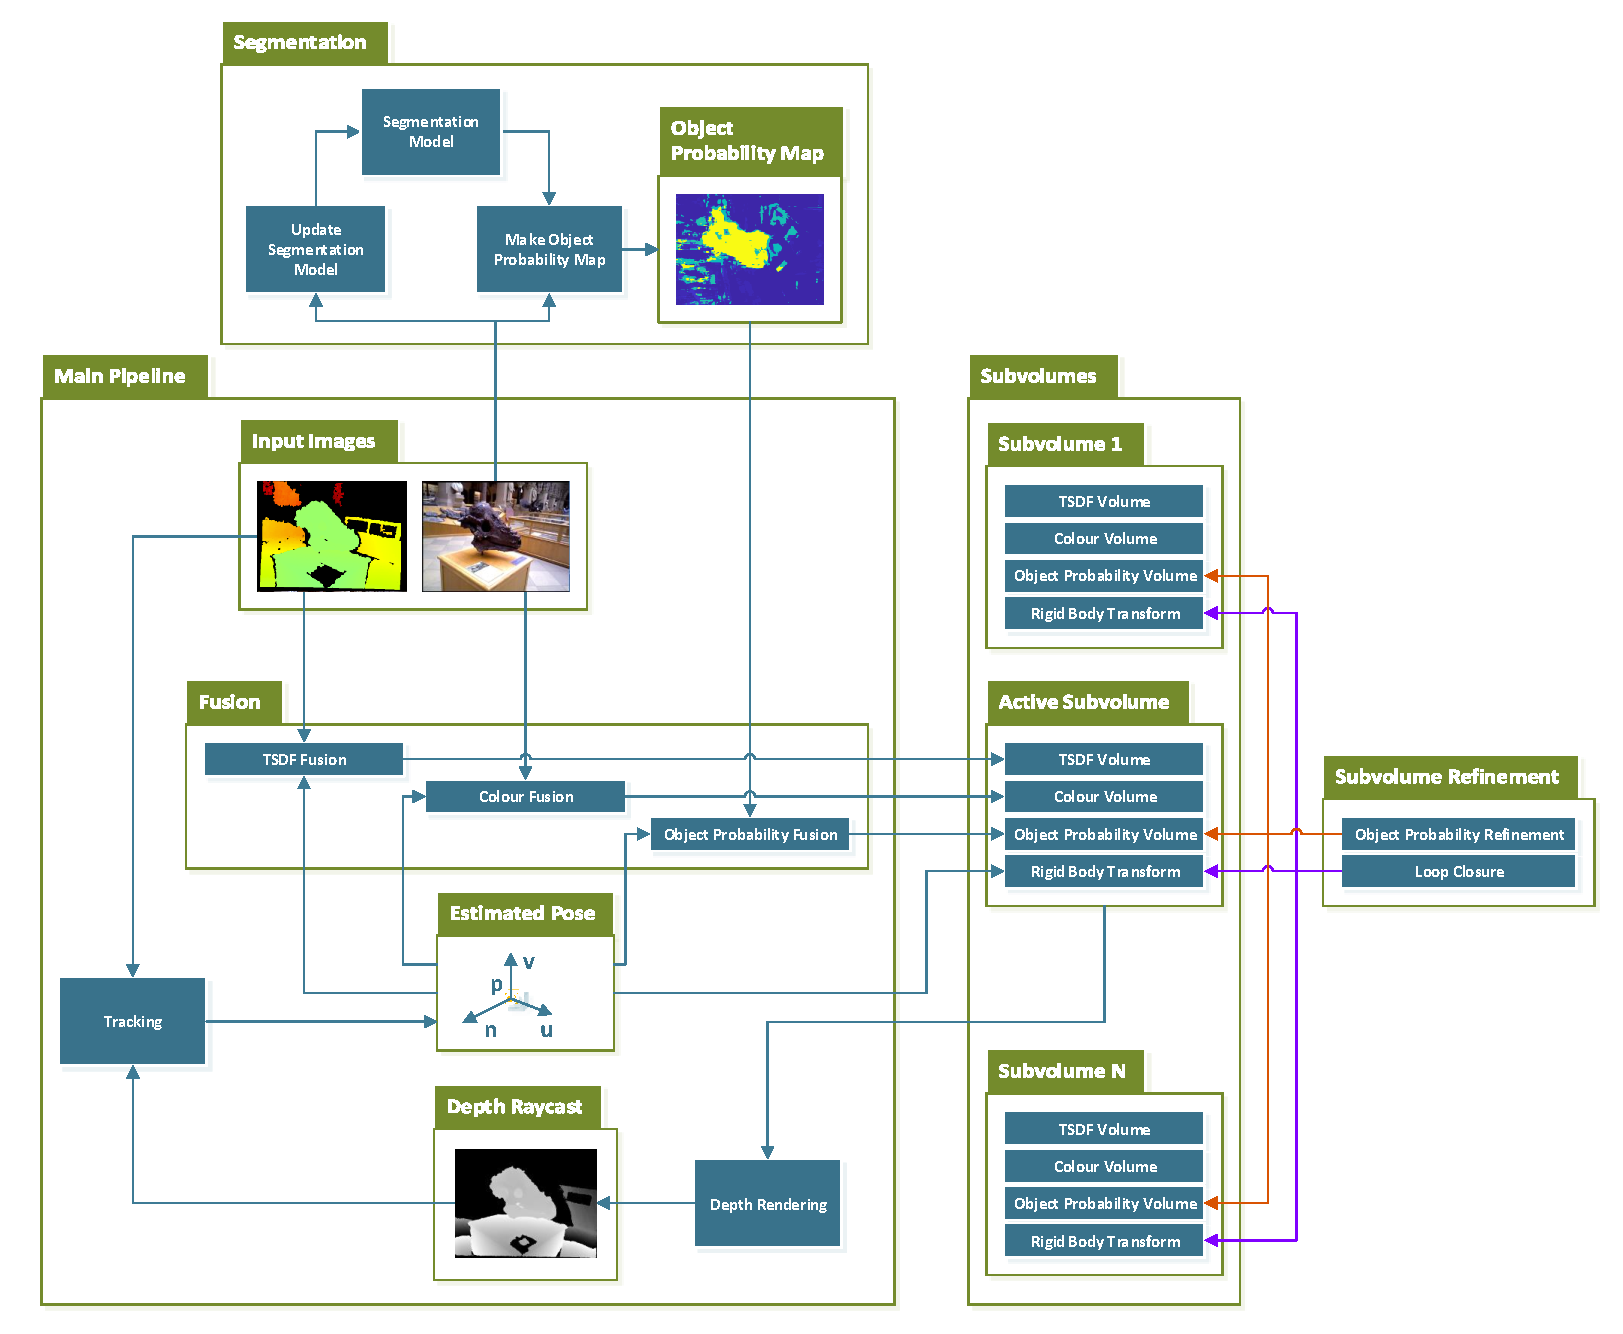
\includegraphics[width=\linewidth]{figures/object_recon/pipeline.pdf}
  \caption{The pipeline of the proposed Object Reconstruction approach.}
\end{figure}

\section{Probabilistic Formulation of Object Reconstruction}


\section{Online Model Correction}

\section{Volumetric Segmentation and Explicit Loop Closure Detection}

\section{Qualitative Results}

\section{Quantitative Results}